\chapter{Analiza techniczna i analiza wymagań}
\label{cha:anaTechIAnaWym}

W rozdziale tym zostaną dokładnie przedstawione oraz porównane mechanizmy lokalnego przechowywania danych po stronie przeglądarki internetowej. Omówiony zostanie również problem dostępności aplikacji w trybie offline oraz używania aplikacji bez dostępnego połączenia internetowego i późniejszej synchronizacji danych.

Ponadto, w rozdziale zostaną przedstawione założenia systemu oraz wymagania które aplikacja powinna spełniać, a także narzędzia oraz technologie które pozwolą na wykonanie aplikacji zgodnie z założonymi wymaganiami.

\section{Lokalne przechowywanie danych}
\label{sec:lokPrzechDanych}

Głównym wymogiem technicznym web aplikacji wspierającej tryb offline jest możliwość użytkowania jej bez konieczności połączenia z serwerem. Do realizacji tego wymogu niezbędne jest przechowywanie danych po stronie klienta - przeglądarki internetowej.

Przechowywanie danych po stronie klienta zawsze było mocną stroną aplikacji desktopowych. W przypadku web aplikacji, przez bardzo długi okres czasu ta funkcjonalność była ograniczona do tworzenia ciasteczek (cookie\cite{cookie}).

Cookie to niewielkie ilości danych każdorazowo przesyłane do serwera przy przeglądaniu danej witryny. Wsparcie przeglądarek dla plików cookie rozpoczęło się w 1995 roku i do drugiej dekady XXI wieku pliki cookie były jedyną szeroko wspieraną metodą przechowywania danych po stronie klienta. Pliki cookie posiadają kilka zasadniczych wad:


\begin{itemize}
\item są przesyłane przy każdym zapytaniu HTTP kierowanym do serwera - niepotrzebnie zwiększenie transferu danych,
\item pliki cookie są przesyłane do serwera niezależnie od użycia protokołu SSL - ryzyko podsłuchania ruchu sieciowego i wycieku danych,
\item rozmiar pliku cookie nie może przekraczać 4KB - brak możliwości przechowywania większych ilości informacji.
\end{itemize}

W przypadku potrzeby uniknięcia ograniczeń cechujących ciasteczka, programista ma do wyboru kilka nowoczesnych metod przechowywania danych po stronie klienta, bazujących na specyfikacji HTML5: WebSQL, Web Storage, IndexedDB, File API. Metody te pozwalają na przechowywanie znacznie większych ilości danych oraz są manualnie przesyłane do serwera, co pozwala na optymalizację zapytań oraz większe bezpieczeństwo danych.

Jednym z kluczowych aspektów w przypadku wyboru metody lokalnego przechowywania danych w web aplikacji jest lista przeglądarek które wspierają daną metodę. O ile w przypadku plików cookie możemy mówić o pełnym wsparciu, o tyle poszczególne metody HTML5 posiadają zróżnicowane poziomy wsparcia zarówno na przeglądarkach desktopowych jak i mobilnych.

\section{Mechanizmy lokalnego przechowywania danych}
\label{sec:mechLokPrzechDanych}

Aby budowa aplikacji www wspierającej tryb offline była możliwa, konieczny jest dobór odpowiedniego mechanizmu lokalnego przechowywania danych. Poniżej, pod względem funkcjonalności, łatwości użytkowania oraz wsparcia na konkretnych przeglądarkach, przeanalizowane zostały obecnie dostępne metody lokalnego przechowywania danych. Z uwagi na niezgodność z wymaganiami funkcjonalnymi aplikacji,  pliki cookie zostały pominięte w poniższej analizie.

\subsection{HTML5 WebSQL Database}
\label{sec:html5WebSqlDatabase}

WebSQL Database\cite{webSqlDb}, jest mechanizmem, który do przechowywania, odczytu oraz aktualizacji danych po stronie klienta wykorzystuje strukturalny język zapytań SQL. Metoda działania mechanizmu bazuje na specyfikacji bazy SQLite. Mechanizm WebSQL posiada zarówno zalety przypisywane relacyjnym bazom danych oraz kilka zalet cechujących metody lokalnego zapisu danych:

\begin{itemize}
\item transakcyjność,
\item łatwość w utrzymaniu integralności danych,
\item dobra wydajność w przypadku wyszukiwania zbioru elementów,
\item szerokie spektrum zastosowań,
\item rozmiar bazy danych ograniczony jedynie dostępną przestrzenią dyskową klienta,
\item asynchroniczne wykonywanie zapytań - interfejs użytkownika nie jest blokowany do czasu zwróceniu rezultatu przez bazę danych.
\end{itemize}

Mechanizm WebSQL sprawdzi się dobrze w przypadku z góry zdefiniowanych struktur danych, które nie muszą być często zmieniane. W przypadku konieczności zmiany struktury danych, wymagane jest każdorazowe napisanie skryptu wykonującego zapytania SQL które pozwolą na aktualizację struktury bazy danych.

WebSQL jest metodą posiadającą umiarkowane wsparcie wśród popularnych przeglądarek internetowych. Tablica 2.1 przedstawia wsparcie przeglądarek dla mechanizmu WebSQL zarówno na systemach desktopowych jak i mobilnych:

\begin{table}[h]
\centering
    \begin{tabular}{ | p{8cm} | p{6cm} | }
    \hline
    \textbf{Przeglądarka} & \textbf{Wsparcie (od wersji)} \\ \hline
	Google Chrome & 4.0
	\\ \hline
	Internet Explorer & brak
	\\ \hline
	Mozilla Firefox & konieczność instalacji rozszerzenia
	\\ \hline
	Safari & 3.1
	\\ \hline
	Android Browser & 2.1
	\\ \hline
	Chrome for Android & 35.0
	\\ \hline
	iOS Safari & 3.2
	\\ \hline
    \end{tabular}
	\caption{Wsparcie mechanizmu WebSQL Database w przeglądarkach internetowych.}
\end{table}

Przy wyborze mechanizmu WebSQL jako metody przechowywania danych po stronie klienta należy wziąć pod uwagę fakt, że specyfikacja standardu nie jest dalej rozwijana. Z tego względu, przy wyborze tej technologii należy liczyć się z możliwością utraty wsparcia na przeglądarkach, które w chwili obecnej je zapewniają. Dodatkowo, przeglądarki które w tym momencie nie oferują wsparcia dla tego mechanizmu, nie dodadzą go przy premierze kolejnych ich wersji.

Biorąc pod uwagę powyższe informacje, użytkowanie aplikacji www bazującej na mechanizmie \mbox{WebSQL} po aktualizacji przeglądarki do nowszej wersji może stać się niemożliwe. Stoi to w sprzeczności z wymaganiami funkcjonalnymi aplikacji, dlatego mechanizm ten nie zostanie wykorzystany przy budowie aplikacji wspierającej tryb offline.

\subsection{HTML5 Web Storage}
\label{sec:html5WebStorage}

HTML5 Web Storage\cite{webStorage}, znany również jako DOM Storage, jest mechanizmem, który przechowuje dane w tablicy asocjacyjnej w której klucze oraz wartości są ciągami tekstowymi. W zależności od przeglądarki internetowej, maksymalny rozmiar danych możliwy do zapisu wynosi od 5 do 35 megabajtów danych.

Web Storage udostępnia dwa obszary składowania danych różniące się zasięgiem oraz cyklem życia:

\begin{itemize}
\item \emph{localStorage} - dane są dostępne we wszystkich oknach oraz kartach danej przeglądarki, dane nie są usuwane po zamknięciu przeglądarki,
\item \emph{sessionStorage} - dane dostępne w obrębie jednej karty przeglądarki, usuwane po jej zamknięciu.
\end{itemize}

Największymi zaletami mechanizmu Web Storage jest kompleksowe wsparcie na wszystkich obecnie popularnych przeglądarkach internetowych (Tablica 2.2), jak również łatwość jego obsługi. Pobranie wartości danego elementu następuje synchronicznie poprzez odwołanie się do globalnego obiektu localStorage lub sessionStorage wraz z podaniem w notacji tablicowej klucza (ciągu znakowego) identyfikującego dany element.

\begin{table}[h]
\centering
    \begin{tabular}{ | p{8cm} | p{6cm} | }
    \hline
    \textbf{Przeglądarka} & \textbf{Wsparcie (od wersji)} \\ \hline
	Google Chrome & 4.0
	\\ \hline
	Internet Explorer & 8.0
	\\ \hline
	Mozilla Firefox & 3.5
	\\ \hline
	Safari & 4.0
	\\ \hline
	Android Browser & 2.1
	\\ \hline
	Chrome for Android & 35.0
	\\ \hline
	iOS Safari & 3.2
	\\ \hline
    \end{tabular}
	\caption{Wsparcie mechanizmu Web Storage w przeglądarkach internetowych.}
\end{table}

Prostota mechanizmu Web Storage ma również swoje wady. Największą z nich jest brak możliwości przechowywania zaawansowanych struktur danych w formacie innym niż łańcuch znaków. W takim przypadku konieczna jest serializacja danych przy zapisie oraz ich deserializacja przy odczycie, co w przypadku dużych obiektów może doprowadzić do problemów z wydajnością.

Dużym ograniczeniem metody jest również brak możliwości efektywnego przeszukiwania danych oraz ich indeksowania. W większości przypadków prowadzi to do konieczności iteracji po wszystkich zdefiniowanych elementach. Synchroniczność zapytań oraz konieczność deserializacji otrzymanych danych skutecznie obniżają szybkość wyszukiwania, szczególnie w przypadku dużej ilości przechowywanych obiektów.

Zarówno konsorcjum W3C zajmujące się rozwojem standardu Web Storage, jak i firmy zajmujące się tworzeniem przeglądarek internetowych są zainteresowane umożliwieniem przechowywania bardziej zaawansowanych struktur danych. Pozwoliłoby to na efektywne zastosowanie Web Storage w przypadku złożonych obiektów. Biorąc pod uwagę cykl życia przeglądarek internetowych oraz średni czas potrzebny użytkownikowi na jej aktualizację, uzyskanie szerszego wsparcia dla tej aktualizacji może zająć kilka lat.

Mechanizm Web Storage posiada pełne wsparcie w obecnych klientach sieci www, jednak nie posiada on wydajnej metody przeszukiwania przechowywanych danych, przez co jego wykorzystanie przy budowie aplikacji www wspierającej tryb offline jest niezalecane na tym etapie rozwoju mechanizmu.

\subsection{HTML5 IndexedDB}
\label{sec:html5IndexedDB}

Indexed Database\cite{indexedDb} jest mechanizmem, który powstał na bazie Web Storage oraz WebSQL, łączy cechy obydwu specyfikacji. IndexedDB przechowuje obiekty języka JavaScript w magazynach obiektów (\emph{objectStores}) które są odpowiednikami tabel w relacyjnej bazie danych.

Każdy rekord przetrzymywany w magazynie musi posiadać unikalny klucz główny który może zostać zdefiniowany przez użytkowika lub, w przeciwnym wypadku, zostanie utworzony automatycznie. W celu optymalizacji przeszukiwania zbioru danych, IndexedDB umożliwia zdefiniowanie indeksu na dowolnym z atrybutów przechowywanych obiektów. Znacząco skraca to czas wyszukiwania oraz ilość potrzebnych do tego zasobów.

Podobnie jak w przypadku mechanizmu WebSQL, IndexedDB wykonuje zapytania asynchronicznie, pozwalając na interakcję użytkownika z aplikacją podczas wykonywania zapytań. Mechanizm wspiera również wersjonowanie bazy danych - w przypadku konieczności aktualizacji bazy do nowszej wersji wykonywane są zdefiniowane przez programistę instrukcje, które powinny zapewnić spójność poprzez aktualizację danych znajdujących się w poprzedniej wersji magazynów obiektów.

Ilość miejsca, jaka może zostać przeznaczona na zasoby przechowywane w IndexedDB jest nieograniczona. W przypadku przekroczenia granicznego rozmiaru bazy danych, indywidualnie ustalanego dla danej przeglądarki internetowej, użytkownik musi wyrazić zgodę na zniesienie ograniczenia ilości miejsca przeznaczonego na magazyny obiektów.

Indexed Database posiada dobre wsparcie wśród nowszych wersji popularnych przeglądarek internetowych (Tablica 2.3).

\begin{table}[h]
\centering
    \begin{tabular}{ | p{8cm} | p{6cm} | }
    \hline
    \textbf{Przeglądarka} & \textbf{Wsparcie (od wersji)} \\ \hline
	Google Chrome & 23.0
	\\ \hline
	Internet Explorer & 10.0
	\\ \hline
	Mozilla Firefox & 10.0
	\\ \hline
	Safari & 8.0
	\\ \hline
	Android Browser & 4.4
	\\ \hline
	Chrome for Android & 35.0
	\\ \hline
	iOS Safari & 8.0
	\\ \hline
    \end{tabular}
	\caption{Wsparcie mechanizmu IndexedDB w przeglądarkach internetowych.}
\end{table}

IndexedDB łączy najlepsze funkcjonalności WebSQL oraz Web Storage. Biorąc pod uwagę dobre wsparcie wśród przeglądarkek, szybkie czasy wyszukiwania elementów przy użyciu indeksów oraz możliwość przechowywania obiektów bez konieczności ich serializacji, mechanizm ten spełnia wszystkie wymagania aplikacji www wspierającej tryb offline.

\subsection{HTML5 Filesystem API}
\label{sec:html5filesystemApi}

Filesystem API\cite{filesystemApi} jest mechanizmem który umożliwia operacje na plikach znajdujących się w wydzielonej przestrzeni na dysku twardym użytkownika. Aby zapis na dysku był możliwy, użytkownik musi najpierw upoważnić do tego aplikację, co odbywa się poprzez zaakceptowanie okna dialogowego wyświetlającego żądanie przechowywania konkretnej ilości danych, jaką dana aplikacja zamierza wykorzystać.

Lista funkcji udostępnianych przez Filesystem API obejmuje zarówno operacje na plikach - zapis, odczyt pliku, odczyt metadanych pliku, kopia do wskazanej lokacji, oraz narzędzia do tworzenia drzewa katalogów oraz ich przeszukiwania. Pliki przechowywane na wydzielonej przestrzeni dyskowej mogą później zostać osadzone jako elementy strony www - jedna z metod Filesystem API zwraca pełny adres URL do danego zasobu.

Pomimo wysokiej użyteczności mechanizmu Filesystem API, wsparcie przeglądarkek ograniczna się do Google Chrome oraz Chrome for Android (Tablica 2.4). W związku z niskim zainteresowaniem innych firm zajmujących się rozwijaniem przeglądarek internetowych, organizacja W3C zawiesiła prace nad tym standardem.

\begin{table}[h]
\centering
    \begin{tabular}{ | p{8cm} | p{6cm} | }
    \hline
    \textbf{Przeglądarka} & \textbf{Wsparcie (od wersji)} \\ \hline
	Google Chrome & 12.0
	\\ \hline
	Internet Explorer & brak
	\\ \hline
	Mozilla Firefox & brak
	\\ \hline
	Safari & brak
	\\ \hline
	Android Browser & brak
	\\ \hline
	Chrome for Android & 35.0
	\\ \hline
	iOS Safari & brak
	\\ \hline
    \end{tabular}
	\caption{Wsparcie mechanizmu Filesystem API w przeglądarkach internetowych.}
\end{table}

Filesystem API jest bardzo dobrym rozwiązaniem dla aplikacji, które wymagają przechowywania dużej ilości zasobów - plików audio, wideo, zdjęć, dokumentów. W przypadku aplikacji które przechowują dane strukturalne, metody WebSQL oraz IndexedDB okażą się dużo bardziej efektywne. Ze względu na niskie wsparcie przeglądarek oraz zawieszenie prac nad rozwojem specyfikacji Filesystem, mechanizm ten nie spełnia wymagań stawianych aplikacji www wspierającej tryb offline.

\section{Aplikacje webowe trybu offline}
\label{sec:appWebOff}

Tryb offline\cite{whatOffline} (w wolnym tłumaczeniu: ,,bez dostępu do sieci Internet") nie był dotychczas kojarzony z przeglądarkami internetowymi - programami z definicji służącymi do przeglądania zasobów WWW (\emph{World Wide Web}). Aplikacje pracujące w tym trybie mogły być wywoływane jedynie poprzez ścieżkę rozpoczynającą się od \textbf{file://} i odwoływać się do danych znajdujących się na dysku twardym, flash lub płycie CD/DVD. Przykładem mogą być prezentacje korzystające z przeglądarki celem uruchomienia animacji napisanych za pomocą języka JavaScript.

Tryb offline pojawia się obecnie również w tak zwanych \textbf{Single-page applications}. Ich działanie polega na wykorzystaniu funkcji przeglądarki internetowej do interakcji z użytkownikiem i zapisania danych lokalnie. Przykład stanowić może TiddlyWiki\footnote{http://tiddlywiki.com/} - osobiste wiki umożliwiające tworzenie i edytowanie treści poprzez uruchomienie pojedynczej strony w przeglądarce bez dostępu do sieci Internet. Cel ten może zostać osiągnięty dzięki dobrodziejstwom oferowanym przez specyfikację HTML5.

Dochodzimy wreszcie do aplikacji wspierających zarówno tryb offline jak i online. Koncepcja ta wykorzystana jest w niniejszej pracy.

Często zasadność tworzenia aplikacji działającej bez dostępu do sieci jest poddawana w wątpliwość. Ogólnodostępność Internetu sprawia, że nawiązanie połączenia nie stanowi obecnie żadnej trudności.

Pomimo prawdziwości powyższego stwierdzenia należy brać pod uwagę względy oszczędnościowe i lokalizacyjne. Mobilność a co za tym idzie ciągła synchronizacja aplikacji zainstalowanych na urządzeniach przenośnych powoduje wzrost zużycia energii. Ponadto nadal istnieją miejsca, gdzie dostęp do sieci Internet jest zabroniony (pokład samolotu) znacząco utrudniony lub nawet niemożliwy.

Poniżej przedstawimy główne prawidłowości działania trybu offline przez pryzmat przeglądarek internetowych.

\subsection{Pamięć cache}
\label{sec:pamiecCache}

Pamięć podręczna przeglądarki\cite{pamiecPodreczna} (ang. \emph{cache}) obejmuje miejsce na dysku twardym przeznaczone do przechowywania odwiedzonych stron WWW lub ich fragmentów. Najczęściej dotyczy to arkuszy stylów CSS, grafik a także skryptów w języku JavaScript. Wyróżniamy dwa główne powody stosowania cache-owania:

\begin{itemize}
\item \textbf{redukcja czasu dostępu do zasobów:} pamięć cache jest znacznie ,,bliżej"{} klienta, niż serwer oryginalny, dzięki czemu w krótszym czasie uzyskiwany jest dostęp do konkretnego zasobu i jego prezentacja,
\item \textbf{redukcja ruchu sieciowego:} przechowywane w pamięci podręcznej zasoby mogą zostać użyte ponownie, co zmniejsza rozmiar pasma niezbędnego do uzyskania dostępu i oszczędza koszty ponoszone przez użytkownika.
\end{itemize}

Pamięć cache dokonuje aktualizacji przechowywanych treści najczęściej raz na sesję (za rozpoczęcie sesji przyjmujemy uruchomienie przeglądarki) tak, by użytkownik był na bieżąco ze zmianami treści. Poniżej przedstawiono ogólne zasady działania Web Cache\cite{cache}:

\begin{enumerate}
\item Działaniem cache sterują nagłówki HTTP. Użytkownik może zdecydować między innymi o czasie przechowywania ,,świeżej"{} porcji danych w pamięci, ich dostępności (private/public) lub nawet o wyłączeniu cache-owania danych.
\item Żądania uwierzytelnienia lub żądania zabezpieczone (np. HTTPS\cite{https}) nie są cache-owane.
\item Reprezentacja danych w cache jest uważana za ,,świeżą"{} (nie musi być sprawdzana z wersją danych na serwerze oryginalnym), jeśli ustawiono nagłówek HTTP odpowiadający za czas życia danych lub jeśli dane były cache-owane niedawno.
\item Jeśli dane są nieaktualne do serwera zostanie wysłane zapytanie o walidację.
\item W sytuacji utraty połączenia internetowego pamięć cache może wysyłać dane bez weryfikacji ich z danymi pochodzącymi z oryginalnego serwera.
\end{enumerate}

W przypadku braku dostępu do nagłówków HTTP możliwa jest edycja ustawień pamięci cache za pomocą znaczników \textbf{meta} zawartych w sekcji head definicji dokumentu HTML.

Proces zapisywania w pamięci podręcznej jest w dużej mierze zautomatyzowany i związany z wyświetleniem witryny. Należy rozgraniczyć na czym polegać, w kontekście projektu, będzie przechowywanie lokalne.

Użytkownik manualnie wywoła proces zapisu danych wykonując akcje na interfejsie aplikacji jak na przykład dodanie/edycja/usunięcie wydarzenia, edycja ustawień etc. Bez ingerencji dane nie trafią do pamięci podręcznej w odróżnieniu od cache-owania wykonywanego automatycznie podczas wyświetlenia dokumentu HTML.

\subsection{Detekcja połączenia sieciowego}
\label{sec:detPolSieciowego}

Wymogiem działania aplikacji jest automatyczna detekcja połączenia internetowego i przejście do trybu online/offline. Jest to spowodowane koniecznością uruchomienia zapisu lokalnego lub synchronizacji danych do serwera aplikacji.

Specyfikacja HTML5 oferuje różne mechanizmy wykrywania połączenia sieciowego. Różnią się one poziomem wsparcia w przeglądarkach.

Jednym z nich jest skorzystanie z tzw. Obserwatora Zdarzeń (\emph{EventListener})\cite{html5off}. HTML5 udostępnia obserwatory \textbf{online} oraz \textbf{offline}.

Połączenie internetowe może także zostać zweryfikowane za pomocą obiektu \textbf{XMLHttpRequest (XHR)}\cite{xhr}. Jest to obiekt języków skryptowych (jak np. JavaScript) umożliwiający wykonanie żądań po załadowaniu się dokumentu HTML. Są one realizowane asynchronicznie (w tle) i nie przerywają interakcji użytkownika ze stroną. Badanie dostępu do Internetu ogranicza się do sprawdzenia odpowiedzi z serwera.

Biblioteką również wykorzystującą technologię AJAX (\emph{Asynchronous JavaScript and XML}) w detekcji połączenia jest Offline.js. Umożliwia ona wykrycie utraconego połączenia oraz ponowne wykonanie żądań, które w wyniku owej utraty nie doszły do skutku. Dodatkowo oferuje szablony służące do wyświetlenia odpowiednich informacji dla użytkownika.

Szczegóły zastosowanych mechanizmów zostaną omówione w rozdziałach poświęconych projektowi i implementacji systemu.

\section{Replikacja i synchronizacja danych}
\label{sec:repIsynchDanych}

Niezbędnym elementem aplikacji www wspierającej tryb offline jest mechanizm  przechowywania danych po stronie klienta. W momencie zerwania połączenia sieciowego  i utraty komunikacji z serwerem, użytkownik powinien posiadać lokalną replikę danych znajdujących się na serwerze. W replice tej powinny zostać zapisane wszystkie wykonane przez niego akcje.

W chwili uzyskania ponownego dostępu do sieci, dane przechowywane w lokalnej bazie danych muszą zostać zsynchronizowane z danymi znajdującymi się na serwerze aby możliwa była ich dalsza propagacja do pozostałych urządzeń z których korzysta dany użytkownik.

Aby aplikacja była w stanie wykonać powyższe zadania, konieczne jest dobór odpowiedniej metody replikacji oraz sychronizacji danych, która pozwoli na stabilne i spójne działanie aplikacji, niezależnie od akcji wykonywanych przez użytkownika oraz stanu połączenia sieciowego.

\subsection{Podstawowe pojęcia}
\label{sec:podstPojecia}

\textbf{Replikacja danych} jest procesem w którym operacje wykonane na danej instacji bazy danych są powielane na pozostałych instancjach objętych mechanizmem replikacji. Głównym celem replikacji jest zwiększenie dostępności oraz szybkości usług sieciowych. Dostępność jest zwiększona poprzez możliowść dostępu do danych w przypadku gdy dostępna jest tylko część replik. Szybkość usług jest zwiększona poprzez dostęp użytkowników do najbliższej, względem ich lokacji, repliki. Prowadzi to do mniejszego opóźnienia sieciowego oraz rozłożenia obciążenia pomiędzy poszczególne repliki wchodzące w skład systemu.

W przypadku aplikacji www wspierających tryb offline mamy do czynienia z przypadkiem, gdy mechanizm lokalnego przechowywania danych obsługiwany przez przeglądarkę użytkownika staje się jedną z replik danych.

\textbf{Transakcją} nazywamy zbiór operacji na bazie danych, które tworzą pewną całość. Aby zmiany wprowadzone przez transakcję zostały zapisane w bazie danych, wszystkie operacje składające się na transakcję muszą zostać poprawnie wykonane. Transakcje powinny spełniać warunki opisane w zasadach ACID (Atomowość, Spójność, Izolacja, Trwałość):

\begin{itemize}
\item Atomowość - w przypadku niepowodzenia przynajmniej jedenej operacji wchodzącej w skład transakcji cała transakcja jest anulowana, pozostawiając dane w niezmienionej formie,
\item Spójność - przed, w trakcie oraz po wykonaniu transakcji system pozostaje w spójnym stanie i nie naruszona zasady integralności danych,
\item Izolacja - w przypadku wielu transakcji wykonywanych współbieżnie, zmiany dokonywane przez poszczególne transakcje są widoczne tylko i wyłącznie z perspektywy danej transakcji.
\item Trwałość - w przypadku awarii, dane wszystkich transakcji które zostały zatwierdzone są zapisane w systemie i będą dostępne po ponownym jego uruchomieniu.
\end{itemize}

\textbf{Szeregowalność} jest pożądaną własnością systemów bazodanowych, która umożliwia zarządzanie operacjami wykonywanymi współbieżnie na bazie danych w taki sposób, aby wyeliminować niepożądane interakcje między nimi. Szeregowalność zapewnia taki sam stan końcowy danych po współbieżnym wykonaniu danych transakcji, jak i po wykonaniu tych transakcji szeregowo.

\textbf{Zakleszczenie} jest zdarzeniem, które zachodzi w sytuacji gdy dwa procesy, każdy z nich wykonujący transakcję, modyfikują wspólny zbiór rekordów w odwrotnej kolejności. Prowadzi to do sytuacji, w której każdy z procesów czeka na zakończenie przeciwnego, co w przypadku zakleszczenia nie następuje. System zarządzania bazą danych odpowiada za wykrywanie zakleszczeń i ich rozwiązywanie, zazwyczaj przez anulowanie jednej z transakcji.

\subsection{Klasyfikacja technik replikacji}
\label{sec:klasTechReplik}

Istnieje wiele technik replikacji które pozwalają na skuteczną oraz stabilną pracę rozproszonych systemów bazodanowych. Główne cechy replikacji które muszą zostać określone to:

\begin{itemize}
\item zakres replikowanych danych,
\item sposób sychronizacji pomiędzy węzłami,
\item poziom dostępu do danych w zależności od statusu repliki.
\end{itemize}

Poniżej przedstawione zostały klasyfikacje które pomagą określić typ replikacji, który oferuje najlepszą funkcjonalność w przypadku aplikacji www wspierających tryb offline.

\setlength{\parskip}{10pt plus 1pt minus 1pt}
\textbf{Replikacja całościowa - Replikacja częściowa}
\setlength{\parskip}{10pt plus 1pt minus 1pt}

Replikacja całościowa zapewnia dostępność pełnej kopii danych na wszystkich węzłach wchodzących w skład systemu.

Replikacja częściowa pozwala na wybór danych, które będą replikowane, przy czym zbiór danych podlegających replikacji jest określany indywidualnie dla każdego węzła wchodzącego w skład systemu. Replikacja częściowa może dzielić zbiór danych na dwa sposoby:

\begin{itemize}
\item horyzontalnie - z danej tabeli wybrany jest zbiór wierszy zawierający wszystkie wartości dla kolumn zdefiniowanych w tej tabeli.
\item wertykalnie - z danej dabeli wybrany jest zbiór kolumn, których wartości dla każdego wiersza są replikowane.
\end{itemize}

\setlength{\parskip}{10pt plus 1pt minus 1pt}
\textbf{Replikacja synchroniczna - Replikacja asynchroniczna}
\setlength{\parskip}{10pt plus 1pt minus 1pt}

Replikacja synchroniczna, tzw. ,,gorliwa", stara się utrzymać zsynchronizowane dane pomiędzy wszystkimi węzłami wchodzącymi w skład systemu. W przypadku replikacji synchronicznej, w skład transakcji wchodzi propagacja danych do wszystkich węzłów - w przypadku wystąpienia konfliktu transakcja jest anulowana. Zapewnia to ochronę przed możliwymi niespójnościami w bazie danych, jednak ryzyko zakleszczenia znacząco wzrasta wraz ze wzrostem liczby transakcji.

Replikacja asynchroniczna, tzn. ,,leniwa", pozwala na niezależne wykonywanie transakcji na każdym z węzłów. Po wykonaniu transakcji na jednym z węzłów, dane są asynchronicznie propagowane do pozostałych węzłów. Replikacja leniwa nie wymaga wysokiej dostępności węzłów, jednak może prowadzić do konfliktów.

Przykładem obrazującym różnicę pomiędzy replikacją leniwą a replikacją gorliwą może być próba wykonania dwóch przelewów z dwóch różnych węzłów objętych replikacją, gdzie obciążenie rachunku przekracza dostępne saldo. W przypadku replikacji gorliwej, pierwsza z transakcji zostanie wykonana pomyślnie, druga zwróci komunikat błędu. W przypadku replikacji leniwej, obie transakcje zakończą się sukcesem, jednak w fazie synchronizacji danych dojdzie do konfliktu, który będzie musiał zostać obsłużony.

\setlength{\parskip}{10pt plus 1pt minus 1pt}
\textbf{Replikacja pesymistyczna - Replikacja optymistyczna}
\setlength{\parskip}{10pt plus 1pt minus 1pt}

Replikacja pesymistyczna zakłada, że stan obiektów przechowywanych w każdym węźle jest identyczny oraz aktualny. W celu uniknięcia konfliktów, w przypadku nieaktualnego stanu danych w węźle, dostęp do danych jest blokowany.

Replikacja optymistyczna nie ogranicza w żaden sposób dostępu do danych, niezależnie od stanu w którym znajduje się replika. Każda z replik przechowuje historię wykonanych transakcji. Ze względu na niezależne wykonywanie transakcji na każdym węźle, w momencie synchronizacji system jest narażony na możliwe konflikty danych. Prowadzi to do konieczności modyfikacji części transakcji i ponownego ich wykonania, co może skutkować innym stanem bazy danych po zakończeniu synchronizacji.

\subsection{Replikacja danych w aplikacji www wspierającej tryb offline}
\label{sec:replDanWAplWWWWspTrybOffline}

Aplikacja www wspierająca tryb offline powinna minimalizować ilość danych przesyłanych pomiędzy poszczególnymi węzłami systemu. Ze względu na prywatność danych, lokalna replika powinna posiadać wyłącznie dane powiązane z konkretnym, zalogowanym w danym momencie do aplikacji, użytkownikiem. Dodatkowo, uwzględniając coraz większą aktywność użytkowników korzystających z urządzeń mobilnych, aplikacja powinna ograniczyć ilość przesyłanych danych do minimum. Z tego względu, replikacja częściowa jest w tym przypadku znacznie lepszym wyborem od replikacji całościowej.

Z uwagi na wymagania aplikacji www oraz nacisk położony na pełną jej funkcjonalność w trybie offline, synchronizacja danych pomiędzy węzłami powinna odbywać się w sposób ,,leniwy''. Przechowywanie danych w lokalnej replice oraz późniejsza asynchroniczna wymiana informacji pomiędzy węzłami powinna zapewnić bardzo płynną interakcję z interfejsem użytkownika, co jest jednym z wymagań aplikacji.  W przypadku użytkowników posiadających repliki danych na wielu urządzeniach które przez większość czasu są fizycznie wyłączone lub nie posiadają dostępu do sieci, zastosowanie replikacji ''gorliwej'' nie byłoby możliwe.

Użytkownik korzystający z aplikacji na urządzeniu mobilnym może znaleźć się w rejonie o słabym zasięgu sieci telefonicznej. W celu oszczędności energii oraz minimalizacji transferu danych przez sieć mobilną, użytkownik może wyłączyć mobilny transfer danych. W przypadku zastosowania replikacji pesymistycznej, uniemożliwiłoby to komunikację z lokalną repliką danych ze względu na nieosiągalność pozostałych węzłów. Z tego względu w aplikacji www wspierającej tryb offline powinna zostać zastosowana replikacja optymistyczna.

Zastosowanie replikacji posiadającej powyższe cechy może doprowadzić do sytuacji, w których podczas procesu synchronizacji wystąpi konflikt transakcji. Aplikacja powinna posiadać wewnętrzne algorytmy które obsłużą takie sytuacje, zaś w przypadku braku możliwości programatycznej obsługi, użytkownik powinien zostać poinformowany o konflikcie oraz o możliwościach jego rozwiązania.

\section{Analiza wymagań}
\label{sec:analizaWymagan}

Tworzony system służy do zarządzania wydarzeniami użytkownika. Zorganizowany jest on w formie interaktywnego kalendarza. Główną zaletą aplikacji jest pełne wsparcie zarówno trybu online jak i offline co uniezależnia ją od stałego dostępu do sieci Internet. Poniższa analiza sugeruje jedynie możliwe zastosowanie systemu zgodnie z jego
pierwotnymi założeniami, aczkolwiek nie wyklucza innej aktywności. Szczegółowy opis możliwości systemu zawarty jest w treści poniższych podrozdziałów.

\subsection{Wymagania funkcjonalne}
\label{sec:wymFunkcj}

Zadaniem aplikacji jest dodawanie, edycja oraz usuwanie wydarzeń. Przez wydarzenie rozumiemy notatkę składającą się z nazwy, czasu trwania oraz treści. Dzięki zaimplementowanemu systemowi autentykacji każdy użytkownik posiada konto, co jednoznacznie identyfikuje wprowadzone przez niego dane. Ponadto użytkownik ma do dyspozycji system powiadomień o nadchodzących wydarzeniach.

Podane akcje mogą być wykonywane zarówno w trybie offline jak i przy aktywnym połączeniu z siecią Internet. Dane gromadzone lokalnie zostają zsynchronizowane z tymi obecnymi w bazie danych serwera aplikacji w momencie wykrycia połączenia. Sam proces synchronizacji może zakończyć się niepowodzeniem, co zostanie obsłużone automatycznie przez zaimplementowane algorytmy lub manualnie, po uprzednim poinformowaniu użytkownika o problemie.

Krytycznym wymaganiem funkcjonalnym systemu jest zapewnienie integralności danych i zapewnienie ciągłości transakcji pomimo problemów z połączeniem sieciowym. Przejście pomiędzy trybami online/offline powinno być płynne i nie wpływać negatywnie na wydajność interfejsu użytkownika.

Z uwagi na zastosowanie optymistycznej replikacji bazy danych należy zwrócić baczną uwagę na możliwość wystąpienia konfliktów pomiędzy żądaniami i ich obsługę.

Ogół operacji realizowanych w ramach aplikacji przedstawia rysunek 2.1.

\begin{figure}[H]
\centering
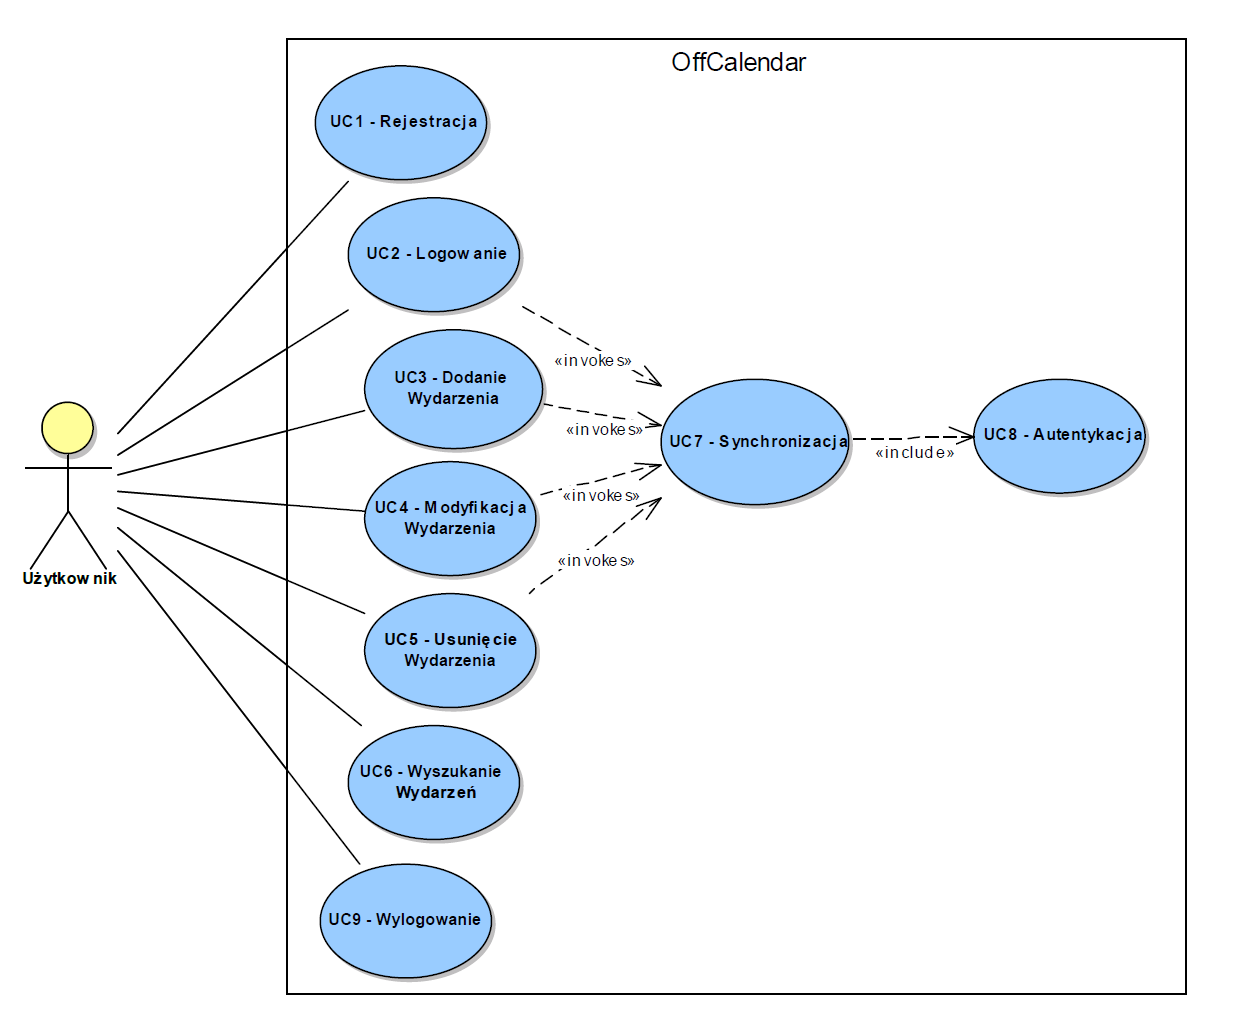
\includegraphics[width=1.0\textwidth]{offcalendar_usecase.png}
\caption{Diagram przypadków użycia aplikacji OffCalendar.}
\end{figure}

Każdy z przypadków użycia (tabele 2.5 - 2.13) składa się z następujących sekcji:

\begin{itemize}
\item identyfikator,
\item tytuł,
\item aktorzy,
\item warunki początkowe,
\item warunki końcowe,
\item cel główny,
\item scenariusz główny,
\item scenariusze alternatywne.
\end{itemize}

\begin{table}[H]
\centering
\begin{tabular}{|l|l|}
	\hline
	\textbf{Identyfikator}                                                                                                                                                                                                                	& UC1                                                                                                                                                                                                                                   	\\ \hline
	\textbf{Tytuł}                                                                                                                                                                                                                        	& Rejestracja użytkownika                                                                                                                                                                                                               	\\ \hline
	\textbf{Aktorzy}                                                                                                                                                                                                                      	& Użytkownik                                                                                                                                                                                                                            	\\ \hline
	\multicolumn{2}{|l|}{\begin{tabular}[c]{@{}l@{}}\textbf{Warunki początkowe:}\\ 1. Użytkownik posiada aktywne połączenie internetowe.\end{tabular}}                                                                                                                                                                                                                                                                                                                             	\\ \hline
	\multicolumn{2}{|l|}{\begin{tabular}[c]{@{}l@{}}\textbf{Warunki końcowe:}\\ 1. Utworzone konto użytkownika zostaje zapisane w bazie danych.\end{tabular}}                                                                                                                                                                                                                                                                                                                                         	\\ \hline
	\multicolumn{2}{|l|}{\begin{tabular}[c]{@{}l@{}}\textbf{Cel główny:}\\ Założenie nowego konta użytkownika w aplikacji OffCalendar.\end{tabular}}                                                                                                                                                                                                                                                                                                                                       	\\ \hline
	\multicolumn{2}{|l|}{\begin{tabular}[c]{@{}l@{}}\textbf{Scenariusz główny:}
	\\1. Użytkownik wpisuje adres URL prowadzący do widoku rejestracji w aplikacji OffCalendar.
	\\2. Użytkownik wypełnia formularz rejestracji składający się z nazwy użytkownika,\\adresu e-mail oraz hasła.
	\\3. Użytkownik przesyła formularz do aplikacji OffCalendar.
	\\4. System wyświetla komunikat potwierdzający rejestrację.
	\\5. System przekierowuje użytkownika do strony logowania.\end{tabular}} 
	\\\hline
	\multicolumn{2}{|l|}{\begin{tabular}[c]{@{}l@{}}\textbf{Scenariusze alternatywne:}
	\\1.A Silnik walidujący dane stwierdził niedozwolone bądź niepoprawne wartości pól\\formularza rejestracyjnego.
	\\\hspace{0.5cm}1.A.1 Aplikacja wyświetla informacje o błędach.
	\\\hspace{0.5cm}1.A.2 Powrót do kroku 2.
	\\1.B Podany w formularzu adres e-mail jest już w użyciu.
	\\\hspace{0.5cm}1.B.1 Aplikacja wyświetla informacje o błędzie.
	\\\hspace{0.5cm}1.B.2 Powrót do kroku 2.
	\end{tabular}}                                                            
	\\ \hline
	\end{tabular}
	\caption{Przypadek użycia UC1: Rejestracja użytkownika.}
\end{table}

\begin{table}[H]
\centering
\begin{tabular}{|l|l|}
	\hline
	\textbf{Identyfikator}                                                                                                                                                                                                                	& UC2
	\\ \hline
	\textbf{Tytuł}                                                                                                                                                                                                                        	& Logowanie użytkownika                                                                                                                                                                                                               	\\ \hline
	\textbf{Aktorzy}                                                                                                                                                                                                                      	& Użytkownik                                                                                                                                                                                                                            	\\ \hline
	\multicolumn{2}{|l|}{\begin{tabular}[c]{@{}l@{}}\textbf{Warunki początkowe:}
	\\1. Użytkownik posiada aktywne połączenie internetowe.
	\\2. Użytkownik posiada konto w aplikacji OffCalendar.
	\\3. Użytkownik posiada przeglądarkę kompatybilną z Web Storage oraz IndexedDB.
	\end{tabular}}                                                                                                                                                                                                                                                                                                                            
 	\\ \hline
	\multicolumn{2}{|l|}{\begin{tabular}[c]{@{}l@{}}\textbf{Warunki końcowe:}
	\\1. Dane użytkownika są zapisane w Web Storage przeglądarki internetowej.\\\end{tabular}}                                                                                                                                                                                                                                                                                                                                         	\\ \hline
	\multicolumn{2}{|l|}{\begin{tabular}[c]{@{}l@{}}\textbf{Cel główny:}\\ Zalogowanie się danego użytkownika w aplikacji OffCalendar.\end{tabular}}                                                                                                                                                                                                                                                                                                                                       	\\ \hline
	\multicolumn{2}{|l|}{\begin{tabular}[c]{@{}l@{}}\textbf{Scenariusz główny:}
	\\1. Użytkownik przechodzi pod adres strony głównej aplikacji OffCalendar.
	\\2. Użytkownik wypełnia formularz logowania składający się z adresu e-mail oraz hasła.
	\\3. Użytkownik przesyła formularz do aplikacji OffCalendar.
	\\4. System wyświetla komunikat o pomyślnej autoryzacji.
	\\5. System przekierowuje użytkownika do głównego widoku aplikacji OffCalendar.\end{tabular}} 
	\\\hline
	\multicolumn{2}{|l|}{\begin{tabular}[c]{@{}l@{}}\textbf{Scenariusze alternatywne:}
	\\2.A Silnik walidujący dane stwierdził niedozwolone bądź niepoprawne wartości pól formularza\\logowania.
	\\\hspace{0.5cm}2.A.1 Aplikacja wyświetla informacje o błędach.
	\\\hspace{0.5cm}2.A.2 Powrót do kroku 2.
	\end{tabular}}                                                            
	\\ \hline
	\end{tabular}
	\caption{Przypadek użycia UC2: Logowanie użytkownika.}
\end{table}

\begin{table}[H]
\centering
\begin{tabular}{|l|l|}
	\hline
	\textbf{Identyfikator}                                                                                                                                                                                                                	& UC3                                                                                                                                                                                                                                   	\\ \hline
	\textbf{Tytuł}                                                                                                                                                                                                                        	& Dodanie wydarzenia
	\\ \hline
	\textbf{Aktorzy}                                                                                                                                                                                                                      	& Użytkownik                                                                                                                                                                                                                            	\\ \hline
	\multicolumn{2}{|l|}{\begin{tabular}[c]{@{}l@{}}\textbf{Warunki początkowe:}\\ 1. Użytkownik jest zalogowany w aplikacji OffCalendar.\end{tabular}}                                                                                                                                                                                                                                                                                                                             	\\ \hline
	\multicolumn{2}{|l|}{\begin{tabular}[c]{@{}l@{}}\textbf{Warunki końcowe:}\\ 1. Dane wydarzenia są zapisane w IndexedDB przeglądarki internetowej.\end{tabular}}                                                                                                                                                                                                                                                                                                                                         	\\ \hline
	\multicolumn{2}{|l|}{\begin{tabular}[c]{@{}l@{}}\textbf{Cel główny:}\\ Dodanie nowego wydarzenia w aplikacji OffCalendar.\end{tabular}}                                                                                                                                                                                                                                                                                                                                       	\\ \hline
	\multicolumn{2}{|l|}{\begin{tabular}[c]{@{}l@{}}\textbf{Scenariusz główny:}
	\\1. Użytkownik przechodzi do widoku dziennego z głównego okna aplikacji OffCalendar.
	\\2. Użytkownik wypełnia formularz dodawania wydarzenia składający się z pól: data początkowa,\\data końcowa, treść wydarzenia, zewnętrzny adres URL, typ wydarzenia oraz ,,wysyłaj notyfikacje?".
	\\3. Użytkownik przesyła formularz do aplikacji OffCalendar.
	\\4. System wyświetla komunikat potwierdzający pomyślne dodanie nowego wydarzenia.
	\\5. System przekierowuje użytkownika do strony głównej aplikacji OffCalendar i odświeża dashboard.\end{tabular}} 
	\\\hline
	\multicolumn{2}{|l|}{\begin{tabular}[c]{@{}l@{}}\textbf{Scenariusze alternatywne:}
	\\3.A Silnik walidujący dane stwierdził niedozwolone bądź niepoprawne wartości pól formularza\\dodawania nowego wydarzenia.
	\\\hspace{0.5cm}3.A.1 Aplikacja wyświetla informacje o błędach.
	\\\hspace{0.5cm}3.A.2 Powrót do kroku 2.
	\end{tabular}}                                                            
	\\ \hline
	\end{tabular}
	\caption{Przypadek użycia UC3: Dodanie wydarzenia.}
\end{table}

\begin{table}[H]
\centering
\begin{tabular}{|l|l|}
	\hline
	\textbf{Identyfikator}                                                                                                                                                                                                                	& UC4                                                                                                                                                                                                                                   	\\ \hline
	\textbf{Tytuł}                                                                                                                                                                                                                        	& Modyfikacja wydarzenia
	\\ \hline
	\textbf{Aktorzy}                                                                                                                                                                                                                      	& Użytkownik                                                                                                                                                                                                                            	\\ \hline
	\multicolumn{2}{|l|}{\begin{tabular}[c]{@{}l@{}}\textbf{Warunki początkowe:}
	\\ 1. Użytkownik jest zalogowany w aplikacji OffCalendar.
	\\ 2. Użytkownik dodał przynajmniej jedno wydarzenie w aplikacji OffCalendar.	
	\end{tabular}}                                                                                                                                                                                                                                                                                                                             	\\ \hline
	\multicolumn{2}{|l|}{\begin{tabular}[c]{@{}l@{}}\textbf{Warunki końcowe:}\\ 1. Dane wydarzenia są zapisane w IndexedDB przeglądarki internetowej.\end{tabular}}                                                                                                                                                                                                                                                                                                                                         	\\ \hline
	\multicolumn{2}{|l|}{\begin{tabular}[c]{@{}l@{}}\textbf{Cel główny:}\\ Modyfikacja wydarzenia w aplikacji OffCalendar.\end{tabular}}                                                                                                                                                                                                                                                                                                                                       	\\ \hline
	\multicolumn{2}{|l|}{\begin{tabular}[c]{@{}l@{}}\textbf{Scenariusz główny:}
	\\1. Użytkownik przechodzi do sekcji modyfikacji poprzez kliknięcie przycisku ,,edit" w polu\\modyfikowanego wydarzenia.
	\\2. Użytkownik wypełnia formularz dodawania wydarzenia składający się z pól: data początkowa,\\data końcowa, treść wydarzenia, zewnętrzny adres URL, typ wydarzenia oraz ,,wysyłaj notyfikacje?".
	\\3. Użytkownik przesyła formularz do aplikacji OffCalendar.
	\\4. System wyświetla komunikat potwierdzający pomyślną modyfikację nowego wydarzenia.
	\\5. System przekierowuje użytkownika do strony głównej aplikacji OffCalendar i odświeża dashboard.\end{tabular}} 
	\\\hline
	\multicolumn{2}{|l|}{\begin{tabular}[c]{@{}l@{}}\textbf{Scenariusze alternatywne:}
	\\4.A Silnik walidujący dane stwierdził niedozwolone bądź niepoprawne wartości pól formularza\\modyfikacji wydarzenia.
	\\\hspace{0.5cm}4.A.1 Aplikacja wyświetla informacje o błędach.
	\\\hspace{0.5cm}4.A.2 Powrót do kroku 2.
	\end{tabular}}                                                            
	\\ \hline
	\end{tabular}
	\caption{Przypadek użycia UC4: Modyfikacja wydarzenia.}
\end{table}

\begin{table}[H]
\centering
\begin{tabular}{|l|l|}
	\hline
	\textbf{Identyfikator}                                                                                                                                                                                                                	& UC5
	\\ \hline
	\textbf{Tytuł}                                                                                                                                                                                                                        	& Usunięcie wydarzenia
	\\ \hline
	\textbf{Aktorzy}                                                                                                                                                                                                                      	& Użytkownik                                                                                                                                                                                                                            	\\ \hline
	\multicolumn{2}{|l|}{\begin{tabular}[c]{@{}l@{}}\textbf{Warunki początkowe:}
	\\ 1. Użytkownik jest zalogowany w aplikacji OffCalendar.
	\\ 2. Użytkownik dodał przynajmniej jedno wydarzenie w aplikacji OffCalendar.	
	\end{tabular}}                                                                                                                                                                                                                                                                                                                             	\\ \hline
	\multicolumn{2}{|l|}{\begin{tabular}[c]{@{}l@{}}\textbf{Warunki końcowe:}\\ 1. Dane o usuniętym wydarzeniu są zapisane w IndexedDB przeglądarki internetowej.\end{tabular}}                                                                                                                                                                                                                                                                                                                                         	\\ \hline
	\multicolumn{2}{|l|}{\begin{tabular}[c]{@{}l@{}}\textbf{Cel główny:}\\ Usunięcie wydarzenia z aplikacji OffCalendar.\end{tabular}}                                                                                                                                                                                                                                                                                                                                       	\\ \hline
	\multicolumn{2}{|l|}{\begin{tabular}[c]{@{}l@{}}\textbf{Scenariusz główny:}
	\\1. Użytkownik przechodzi do sekcji usuwania wydarzenia poprzez kliknięcie przycisku ,,delete" w polu\\usuwanego wydarzenia.
	\\2. System przekierowuje użytkownika do strony głównej aplikacji OffCalendar i odświeża dashboard.\end{tabular}} 
	\\\hline
	\multicolumn{2}{|l|}{\begin{tabular}[c]{@{}l@{}}\textbf{Scenariusze alternatywne:}
	\\brak
	\end{tabular}}                                                            
	\\ \hline
	\end{tabular}
	\caption{Przypadek użycia UC5: Usunięcie wydarzenia.}
\end{table}

\begin{table}[H]
\centering
\begin{tabular}{|l|l|}
	\hline
	\textbf{Identyfikator}                                                                                                                                                                                                                	& UC6
	\\ \hline
	\textbf{Tytuł}                                                                                                                                                                                                                        	& Wyszukiwanie wydarzeń
	\\ \hline
	\textbf{Aktorzy}                                                                                                                                                                                                                      	& Użytkownik                                                                                                                                                                                                                            	\\ \hline
	\multicolumn{2}{|l|}{\begin{tabular}[c]{@{}l@{}}\textbf{Warunki początkowe:}
	\\ 1. Użytkownik jest zalogowany w aplikacji OffCalendar.
	\end{tabular}}                                                                                                                                                                                                                                                                                                                             	\\ \hline
	\multicolumn{2}{|l|}{\begin{tabular}[c]{@{}l@{}}\textbf{Warunki końcowe:}\\brak\end{tabular}}                                                                                                                                                                                                                                                                                                                                         	\\ \hline
	\multicolumn{2}{|l|}{\begin{tabular}[c]{@{}l@{}}\textbf{Cel główny:}\\Wyszukiwanie wydarzeń w aplikacji OffCalendar.\end{tabular}}                                                                                                                                                                                                                                                                                                                                       	\\ \hline
	\multicolumn{2}{|l|}{\begin{tabular}[c]{@{}l@{}}\textbf{Scenariusz główny:}
	\\1. Użytkownik wypełnia formularz wyszukiwania wydarzenia składający się z pola ,,treść wydarzenia".
	\\2. Użytkownik wysyła formularz do aplikacji OffCalendar.
	\\3. System wyświetla listę pasujących wydarzeń.\end{tabular}} 
	\\\hline
	\multicolumn{2}{|l|}{\begin{tabular}[c]{@{}l@{}}\textbf{Scenariusze alternatywne:}
	\\6.A System nie odnalazł wydarzeń pasujących do podanej przez użytkownika frazy.
	\\\hspace{0.5cm}6.A.1 Aplikacja wyświetla informacje o braku wyników wyszukiwania.
	\\\hspace{0.5cm}6.A.2 Powrót do kroku 1.
	\end{tabular}}                                                            
	\\ \hline
	\end{tabular}
	\caption{Przypadek użycia UC6: Wyszukiwanie wydarzeń.}
\end{table}

\begin{table}[H]
\centering
\begin{tabular}{|l|l|}
	\hline
	\textbf{Identyfikator}                                                                                                                                                                                                                	& UC7
	\\ \hline
	\textbf{Tytuł}                                                                                                                                                                                                                        	& Synchronizacja
	\\ \hline
	\textbf{Aktorzy}                                                                                                                                                                                                                      	& Użytkownik                                                                                                                                                                                                                            	\\ \hline
	\multicolumn{2}{|l|}{\begin{tabular}[c]{@{}l@{}}\textbf{Warunki początkowe:}
	\\ 1. Użytkownik jest zalogowany w aplikacji OffCalendar.
	\\ 2. Użytkownik posiada aktywne połączenie internetowe.
	\end{tabular}}                                                                                                                                                                                                                                                                                                                             	\\ \hline
	\multicolumn{2}{|l|}{\begin{tabular}[c]{@{}l@{}}\textbf{Warunki końcowe:}
	\\1. Stemple czasowe wydarzeń zostały zaktualizowane.
	\\2. Stempel czasowy ostatniej synchronizacji został zaktualizowany.\end{tabular}}                                                                                                                                                                                                                                                                                                                                         	\\ \hline
	\multicolumn{2}{|l|}{\begin{tabular}[c]{@{}l@{}}\textbf{Cel główny:}\\Synchronizacja wydarzeń przechowywanych lokalnie z wydarzeniami przechowywanymi na serwerze.\end{tabular}}                                                                                                                                                                                                                                                                                                                                       	\\ \hline
	\multicolumn{2}{|l|}{\begin{tabular}[c]{@{}l@{}}\textbf{Scenariusz główny:}
	\\1. Aplikacja kliencka wysyła do serwera wydarzenia posiadające nowszy stempel czasowy od\\stempla ostatniej synchronizacji.
	\\2. Aplikacja serwerowa zwraca wydarzenia które wymagające synchronizacji po stonie klienta\\oraz stempel czasowy synchronizacji.
	\\3. Aplikacja kliencka aktualizuje lokalnie przechowywane wydarzenia.
	\\4. Aplikacja kliencka odświeża widok dashboard.\end{tabular}} 
	\\\hline
	\multicolumn{2}{|l|}{\begin{tabular}[c]{@{}l@{}}\textbf{Scenariusze alternatywne:}
	\\7.A Autentykacja użytkownika nie powiodła się.
	\\\hspace{0.5cm}7.A.1 Aplikacja kliencka wyświetla informacje o błędach.
	\\\hspace{0.5cm}7.A.2 Koniec procesu.
	\end{tabular}}                                                            
	\\ \hline
	\end{tabular}
	\caption{Przypadek użycia UC7: Synchronizacja.}
\end{table}

\begin{table}[H]
\centering
\begin{tabular}{|l|l|}
	\hline
	\textbf{Identyfikator}                                                                                                                                                                                                                	& UC8
	\\ \hline
	\textbf{Tytuł}                                                                                                                                                                                                                        	& Autentykacja
	\\ \hline
	\textbf{Aktorzy}                                                                                                                                                                                                                      	& Użytkownik                                                                                                                                                                                                                            	\\ \hline
	\multicolumn{2}{|l|}{\begin{tabular}[c]{@{}l@{}}\textbf{Warunki początkowe:}
	\\ 1. Użytkownik posiada aktywne połączenie internetowe.
	\end{tabular}}                                                                                                                                                                                                                                                                                                                             	\\ \hline
	\multicolumn{2}{|l|}{\begin{tabular}[c]{@{}l@{}}\textbf{Warunki końcowe:}\\brak\end{tabular}}                                                                                                                                                                                                                                                                                                                                         	\\ \hline
	\multicolumn{2}{|l|}{\begin{tabular}[c]{@{}l@{}}\textbf{Cel główny:}\\Potwierdzenie tożsamości użytkownika na podstawie przesłanych danych.\end{tabular}}                                                                                                                                                                                                                                                                                                                                       	\\ \hline
	\multicolumn{2}{|l|}{\begin{tabular}[c]{@{}l@{}}\textbf{Scenariusz główny:}
	\\1. Aplikacja kliencka wysyła do serwera dane wymagane przy procesie autentykacji użytkownika.
	\\2. Aplikacja serwerowa weryfikuje tożsamość użytkownika na podstawie przesłanych danych\\(adres e-mail oraz hasło).
	\\3. Aplikacja serwerowa zwraca dane użytkownika.\end{tabular}} 
	\\\hline
	\multicolumn{2}{|l|}{\begin{tabular}[c]{@{}l@{}}\textbf{Scenariusze alternatywne:}
	\\8.A Weryfikacja tożsamości użytkownika nie powiodła się.
	\\\hspace{0.5cm}8.A.1 Aplikacja zwraca kod błędu.
	\\\hspace{0.5cm}8.A.2 Koniec procesu.
	\end{tabular}}                                                            
	\\ \hline
	\end{tabular}
	\caption{Przypadek użycia UC8: Autentykacja.}
\end{table}

\begin{table}[H]
\centering
\begin{tabular}{|l|l|}
	\hline
	\textbf{Identyfikator}                                                                                                                                                                                                                	& UC9
	\\ \hline
	\textbf{Tytuł}                                                                                                                                                                                                                        	& Wylogowanie użytkownika
	\\ \hline
	\textbf{Aktorzy}                                                                                                                                                                                                                      	& Użytkownik                                                                                                                                                                                                                            	\\ \hline
	\multicolumn{2}{|l|}{\begin{tabular}[c]{@{}l@{}}\textbf{Warunki początkowe:}
	\\ 1. Użytkownik jest zalogowany w aplikacji OffCalendar.	
	\end{tabular}}                                                                                                                                                                                                                                                                                                                             	\\ \hline
	\multicolumn{2}{|l|}{\begin{tabular}[c]{@{}l@{}}\textbf{Warunki końcowe:}\\1. Dane użytkownika zostają usunięte z Web Storage przeglądarki internetowej.\end{tabular}}                                                                                                                                                                                                                                                                                                                                         	\\ \hline
	\multicolumn{2}{|l|}{\begin{tabular}[c]{@{}l@{}}\textbf{Cel główny:}\\Wylogowanie użytkownika z aplikacji OffCalendar.\end{tabular}}                                                                                                                                                                                                                                                                                                                                       	\\ \hline
	\multicolumn{2}{|l|}{\begin{tabular}[c]{@{}l@{}}\textbf{Scenariusz główny:}
	\\1. Użytkownik klika przycisk ,,Logout"{} celem wylogowania z systemu.
	\\2. System przekierowuje użytkownika do strony logowania i pozbywa się jego danych zapisanych\\w pamięci podręcznej przeglądarki.\end{tabular}} 
	\\\hline
	\multicolumn{2}{|l|}{\begin{tabular}[c]{@{}l@{}}\textbf{Scenariusze alternatywne:}
	\\brak
	\end{tabular}}                                                            
	\\ \hline
	\end{tabular}
	\caption{Przypadek użycia UC9: Wylogowanie użytkownika.}
\end{table}

\subsection{Wymagania niefunkcjonalne}
\label{sec:wymNieFunkcj}

Projektowany system składa się z dwóch zasadniczych części: aplikacji klienckiej stworzonej w technologii HTML5 oraz części serwerowej złożonej z serwera www oraz bazy danych. Poszczególne komponenty stawiają określone wymagania z uwagi na specyfikę projektu.

Aplikacja kliencka z założenia dedykowana jest przeglądarkom internetowym. Interfejs programu zbudowany został w oparciu o język znaczników HTML5. Za warstwę wizualną odpowiada język kaskadowych arkuszy stylów CSS. Asynchroniczna obsługa systemu możliwa jest dzięki zastosowaniu języka skryptowego JavaScript. Wspomniane rozwiązania umożliwiają stworzenie przejrzystego i responsywnego interfejsu przystosowanego zarówno do przeglądarek desktopowych jak i mobilnych, co stanowi obecnie standard i gwarant wygodnego korzystania z systemu.

Wymogiem dla technologii lokalnego przechowywania danych wprowadzanych przez użytkownika jest możliwość przechowywania stosunkowo złożonych rekordów bez konieczności ich serializacji, szerokie wsparcie wśród przeglądarek oraz szybkie wyszukiwanie. IndexedDB łączy wszystkie wymienione wymagania i stanowi najlepszy wybór wśród obecnie stosowanych technologii. Dodatkowym atutem jest bogata i aktualizowana dokumentacja.

Aplikacja kliencka winna działać na przeglądarkach internetowych oferujących wsparcie dla mechanizmu IndexedDB. Ich lista wraz z minimalnymi wersjami oferującymi wsparcie znajduje się w \textbf{Sekcji 2.2.3}.

Serwer aplikacji wraz z bazą danych gwarantują nieprzerwaną obsługę żądań użytkowników. Dane synchronizowane pomiędzy klientem a serwerem powinny zachować spójność i integralność. W przypadku braku połączenia internetowego komplet wprowadzonych przez użytkownika informacji powinien być dostępny w pamięci podręcznej przeglądarki.

Platforma zapewnia bezpieczną autentykację dla użytkowników posiadających konta.

Komunikacja pomiędzy częściami systemu powinna minimalizować narzut danych celem ograniczenia kosztów transmisji, co motywuje zastosowanie architektury REST wykorzystującej lekki format JSON \emph{(JavaScript Object Notation)}\cite{json}.

Detekcja połączenia sieciowego winna następować automatycznie wraz z przełączeniem się systemu na tryb offline/online.

\section{Wykorzystane technologie i narzędzia}
\label{sec:wykoTechnINarz}

Aby aplikacja www wspierająca tryb offline mogła zostać wykonana, konieczny był dobór odpowiednich narzędzi programistycznych oraz technologii umożliwiających zrealizowanie założonego celu.

Najważniejsze elementy które muszą zostać wykonane w części klienckiej aplikacji to szata graficzna, napisanie kodu HTML tworzącego strukturę interfejsu oraz dodanie odpowiednich reguł w kaskadowych arkuszach stylów tworzących warstwę prezentacji. Aby umożliwić pracę aplikacji w trybie offline, konieczna jest integracja wybranego mechanizmu lokalnego przechowywania danych oraz stworzenie komponentu odpowiedzialnego za synchronizację danych przy użyciu języka JavaScript.

W części serwerowej aplikacji, głównym zadaniem będzie stworzenie struktury bazy danych \mbox{MySQL} przechowującej dane użytkowników, stworzenie usług odpowiadających za komunikację z częścią kliencką aplikacji oraz komponentu odpowiedzialnego za rozwiązywanie konfliktów mogących powstać przy procesie synchronizacji danych.

\subsection{Netbeans IDE}
\label{sec:netbeans}

Netbeans IDE jest zintegrowanym środowiskiem programistycznym posiadającym bardzo dobre wsparcie zarówno dla używanych przez nas technologii serwerowych ( PHP, MySQL, Apache), webowych (HTML, CSS, JavaScript) jak i użytego w projekcie systemu kontroli wersji (GIT). Dodatkowym atutem Netbeans IDE jest jego udostępnianie na licencji GNU General Public License, co czyni oprogramowanie darmowym zarówno w użytku prywatnym jak i komercyjnym.

Alternatywą dla Netbeans IDE jest PHPStorm -- doskonałe środowisko rozwijane przez firmę JetBrains. Posiada ono wszystkie jego zalety, a ponadto oferuje szereg zaawansowanych narzędzi służących do połączenia ze zdalnym serwerem, testowania oraz debugowania rozwijanej aplikacji. PHPStorm nie został wykorzystany w projekcie, ponieważ jest to płatne oprogramowanie, którego dodatkowe narzędzia nie znajdą zastosowania podczas procesu tworzenia aplikacji www wspierającej tryb offline.

\subsection{Adobe Photoshop CS3}
\label{sec:photoshop}

Każda aplikacja www powinno posiadać szatę graficzną dostosowaną do jej potrzeb. Adobe Photoshop jest najpopularniejszym na rynku narzędziem do edycji grafiki rastrowej oraz tworzenia interfejsów strow www. Do największych zalet należy zaliczyć ergonomiczny interfejs, zaawansowane możliwości operacji na warstwach oraz bogaty zestaw efektów, który możemy nadać danemu elementowi. Szybka możliwość eksportu poszczególnych grafik, osadzanych później w kodzie HTML, jest kolejną funkcjonalnością która sprawia że program spełnia wszystkie wymagania.

Alternatywnym oprogramowaniem umożliwiającym edycję grafiki rastrowej jest GIMP (\emph{GNU Image Manipulation Program}). GIMP jest darmowym odpowiednikiem Adobe Photoshop, jednak oferującym znacznie bardziej ograniczone możliwości manipulacji warstwami, tworzenia szablonów oraz nadawania efektów poszczególnym elementom. Niska ergonomia oraz intuicyjność interfejsu sprawia, że czas potrzebny na uzyskanie takiego samego efektu końcowego jak w Adobe Photoshop jest znacznie dłuższy. Z tego względu, mimo darmowej licencji, oprogramowanie GIMP nie zostało wykorzystane w projekcie.

\subsection{HTML5}
\label{sec:html5}

HTML jest podstawowym językiem służącym do tworzenia stron www. Zadaniem znaczników HTML jest nadanie semantycznego znaczenia elementom renderowanym na stronie. Inne zastosowania znaczników obejmują m. in. za załączenie odpowiednich arkuszy stylów, wczytanie bibliotek i skryptów języka JavaScript, określenie sposobu indeksowania strony oraz reguły specyfikujące sposób przechowywania dokumentów w pamięci cache.

Z punktu widzenia aplikacji wspierającej tryb offline, szczególnie ważnymi elementami wywodzącymi się ze specyfikacji HTML5 są mechanizmy lokalnego przechowywania danych oraz instrukcje pozwalające określić metodę przechowywania poszczególnych zasobów strony www w pamięci cache. Dodatkowym atutem języka HTML5 jest natywna walidacja danych wprowadzanych do formularzy przez użytkownika oraz rozszerzony zbiór semantycznych znaczników, pozwalający na trafniejsze opisanie elementów strukturalnych dokumentu, takich jak nagłówek, stopka, nawigacja czy panel boczny.

\subsection{Kaskadowe arkusze stylów}
\label{sec:css}

Kaskadowe arkusze stylów (\emph{CSS - Cascading Style Sheets}) to nieodłączny element stron www. Kaskadowe arkusze stylów zostały zaprojektowane z myślą o separacji warstwy prezentacji strony od jej treści. Poprzez zawarcie reguł opisujących sposób wyświetlania poszczególnych elementów dokumentu HTML w zewnętrznym arkuszu stylów, możliwe jest łatwe ich dołączenie do wszystkich dokumentów. Edycja danej reguły w zewnętrznym pliku CSS powoduje aktualizację wszystkich stron używających danego pliku, co znacznie usprawnia pracę nad większymi projektami.

Reguły w kaskadowych arkuszach stylów mogą zostać załączane warunkowo. Typowym zastosowaniem są tutaj odrębne style dla drukowanych dokumentów. Bardziej zaawansowane reguły pozwalają na zastosowanie odrębnych zestawów reguł w zależności od rozdzielczości ekranu czy też rozmiaru okna przeglądarki. Umożliwia to tworzenie responsywnych interfejsów, zachowujących ergonomię niezależnie od urządzenia na jakim interfejs jest wyświetlony.

\subsection{Skryptowy język programowania JavaScript}
\label{sec:js}

Język JavaScript jest nieodłącznym elementem interaktywnych aplikacji webowych. Szczególnie dużą rolę pełni on w aplikacjach wspierających tryb offline, jako że jest to jedyna technologia która pozwala zastąpić dynamiczną treść generowaną na zdalnym serwerze. Dzieje się to poprzez monitorowanie akcji wykonywanych przez użytkownika aplikacji oraz ich obsługę po stronie przeglądarki internetowej.

Mechanizmy lokalnego przechowywania danych są silnie uzależnione od języka JavaScript. Wszystkie operacje zapisu, odczytu oraz modyfikacji danych obdywają się za jego pośrednictwem, poprzez odwołanie się do obiektów oraz metod wyszczególnionych z specyfikacji danej metody lokalnego przechowywania danych.

W ostatnich latach nastąpił znaczny rozwój frameworków oraz bibliotek języka JavaScript. Udostępniane przez nie narzędzia znacznie ułatwiają pracę nad tworzeniem dynamicznych elementów aplikacji www.

Wśród najpopularniejszych bibliotek ułatwiających manipulację drzewem dokumentu DOM (\emph{Document Object Model}) znajdują się jQuery, Prototype, MooTools. Ze względu na bardzo dobrą dokumentację oraz możliwość łatwego rozszerzenia natywnej funkcjonalności poprzez bogaty zestaw wtyczek, biblioteka jQuery, wraz z dodatkiem jQuery UI, zostanie wykorzystana w projekcie web aplikacji wspierającej tryb offline.

Złożone aplikacje webowe potrzebują bibliotek oferujących rozwiązania tworzące szkielet architektury, która pozwala na logiczny podział modułów aplikacji oraz funkcjonalności przez nią realizowaną. Do najpopularniejszych bibliotek zaliczymy tutaj AngularJS, Cappuccino czy Knockout. Ze względu na specyfikę aplikacji wspierającej tryb offline oraz konieczność stworzenia dedykowanej warstwy odpowiedzialnej za przechowywania oraz synchronizację danych, biblioteki tworzące architekturę aplikacji nie zostaną zastosowane.

\subsection{Apache 2.4.9}
\label{sec:apache}

Aby aplikacja www była osiągalna dla użytkowników, konieczne jest pośrednictwo serwera www. Apache HTTP Server jest obecnie najpopularniejszym serwerem obsługującym aplikacje webowe. Jest udostępniany na licencji open-source oraz posiada wsparcie zarówno na systemach Unix jak i Windows.

Ze względu na udostępniony zestaw popularnych konfiguracji oraz dużą ilość przewodników opisujących poszczególne funkcjonalności serwera, proces instalacji oraz konfiguracji jest skrócony do minimum. Szczególnie ważne jest to przy niewielkich projektach, w których konfiguracja środowiska programistycznego, lokalnego oraz zdalnego serwera powinna pochłaniać jak najmniej czasu.

\subsection{PHP 5.5}
\label{sec:php}

PHP to skryptowy język programowania zaprojektowany pod kątem użycia w aplikacjach webowych. Kod języka PHP nie jest kompilowany, zamiast tego jest on parsowany oraz interpretowany przez interpreter PHP.

Ze względu na przeniesienie ciężaru logiki aplikacji na stronę klienta (JavaScript) technologia serwerowa powinna być możliwie prosta w zastosowaniu, przy czym posiadająca wsparcie dla wszystkich wymaganych funkcjonalności. Część serwerowa aplikacji będzie ograniczała się do podstawowych widoków, warstwy dostępu do bazy danych oraz interfejsów odpowiedzialnych za uwierzytelnienie użytkownika czy też synchronizację danych.

Język PHP oferuje bardzo dobre wsparcie powyższych elementów aplikacji przy jednoczesnej minimalizacji narzutu technologicznego. PHP, w połączeniu z serwerem Apache oraz technologią MySQL, stanowi spójny zestaw technologii pozwalający na bardzo dobrą skalowalność aplikacji, co jest szczególnie ważne w przypadku późniejszej rozbudowy projektu.

\subsection{MySQL 5.6.17}
\label{sec:mysql}

Jednym z kluczowych elementów aplikacji www wspierającej tryb offline jest sposób przechowywania danych po stronie klienta oraz późniejsza ich synchronizacja. Ze względu na strukturę danych oraz wymaganą transakcyjność przy procesie replikacji danych, zastosowanie relacyjnej bazy danych jest tutaj najlepszym rozwiązaniem. Zarówno MySQL jak i PostgreSQL są zaawansowanymi, darmowymi systemami bazodanowymi oferującymi wymaganą funkcjonalność.

Technologia MySQL posiada silnik InnoDB, oferujący bardzo wysoką wydajność w przypadku aktualizacji rekordów znajdujących się w bazie danych. Poprzez zastosowanie blokady na poziomie wierszy, poszczególne procesy dokonujące synchronizacji danych pomiędzy węzłami systemu powinny zapewniać dobrą wydajność, niezależnie od liczby współbieżnych operacji. MySQL posiada również zaawansowany system replikacji, co jest szczególnie ważne w przypadku problemów z przepustowością pojedynczej instancji bazy danych oraz wyczerpaniu możliwości skalowania wertykalnego. Powyższe cechy sprawiają, że system MySQL zostanie zastosowany w budowie aplikacji www wspierającej tryb offline.
